\documentclass[11pt]{article}
\RequirePackage{fullpage}
\RequirePackage[font=small,labelfont=bf]{caption}
\RequirePackage{amsmath,amssymb,amsthm}
\RequirePackage{mathtools}
\RequirePackage{graphicx}
\RequirePackage[normalem]{ulem}
\RequirePackage[hidelinks]{hyperref}
\RequirePackage{subcaption}
\RequirePackage{wasysym}
\RequirePackage{authblk}
\RequirePackage{bm}
\RequirePackage{bbm}
\RequirePackage{tikz}
\RequirePackage{xr}
\externaldocument{temporal-covariance-manuscript}

% line numbers:
\RequirePackage{lineno}
%\modulolinenumbers[5]
%\definecolor{linenogray}{black}{0.75}
%\renewcommand\linenumberfont{\normalfont\tiny\sffamily\color{linenogray}}

% spacing
\RequirePackage{setspace}
%\doublespacing
 
% \RequirePackage[osf]{mathpazo}
\RequirePackage[bibstyle=authoryear,citestyle=authoryear-comp,
                date=year,
                maxbibnames=9,maxnames=5,maxcitenames=2,
                backend=biber,uniquelist=false,uniquename=false,
                % style=apa,
                % sorting=nyt,
                sorting=ynt,
                hyperref=true]{biblatex}
\RequirePackage[colorinlistoftodos]{todonotes}  %disable
\RequirePackage{color}
\RequirePackage{nicefrac}

\newcommand{\gc}[1]{{\it \color{red} #1 } }
\newcommand{\vb}[1]{{\it \color{blue} #1}}
\newcommand{\vbout}[1]{{\it \color{blue} \sout{#1}}}

% a /nonumber you can turn on/off
\newcommand{\nnn}{\nonumber}
%\newcommand{\nnn}{}


\newcommand{\graham}[1]{\todo[size=\scriptsize, color=red!50]{#1}}
\newcommand{\vince}[1]{\todo[size=\scriptsize, color=blue!50]{#1}}

\renewcommand{\P}{\mathbb{P}}
\newcommand{\E}{\mathbb{E}}
\newcommand{\V}{\text{V}}
\newcommand{\cf}{\emph{cf.} }
\DeclareMathOperator{\var}{Var}
\DeclareMathOperator{\cov}{Cov}
\DeclareMathOperator{\T}{{\mathrm{T}}}
\newcommand{\vect}[1]{\mathbf{#1}}
\newcommand{\nssh}{SSH_n}

\newcommand{\chapquote}[2]{\begin{quotation} \textit{#1} \end{quotation} \begin{flushright} - #2\end{flushright} }

\addbibresource{temporal-covariance.bib}

% \title{Linked Selection During Rapid Polygenic Adaptation Creates an Autocovariance Signal Detectable from Temporal Data}
% \title{A temporal signal of polygenic linked selection}
%\title{A Linked Selection Signal During Rapid Polygenic Adaptation from Temporal Data}
% \title{Rapid Polygenic Adaptation Creates a Detectable Signal of Linked Selection in Temporal Data}
\title{Supplementary Figures for The Linked Selection Signature of Rapid Adaptation in Temporal Genomic Data}

\author[$\ast$,$\dag$,$1$]{Vince Buffalo}
\author[$\dag$]{Graham Coop}
\affil[$\ast$]{\footnotesize Population Biology Graduate Group}
\affil[$\dag$]{\footnotesize Center for Population Biology, Department of Evolution and Ecology, University of California, Davis, CA 95616}
\affil[$1$]{\footnotesize Email for correspondence: \href{mailto:vsbuffalo@ucdavis.edu}{vsbuffalo@ucdavis.edu}}

\begin{document}
\maketitle

\counterwithin{figure}{section}
\setcounter{figure}{0}    



\section{Validation of simulation routine}

\begin{figure}[!ht]
  \centering
  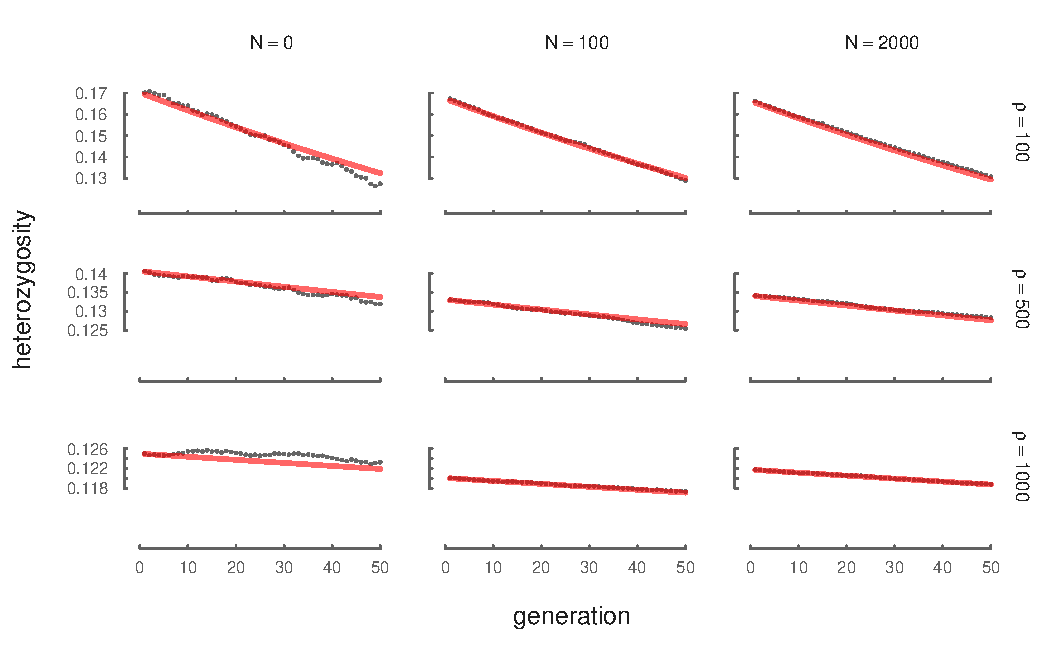
\includegraphics{./images/supp-het-neutral.pdf}

\caption{The neutral decay of heterozygosity due to drift, averaged across 100
replicates and a variety of $N$ and $\rho$ levels. The red line is the
theoretical expectation $H_t = H_1 (1-1/(2N))^{t-1}$.}

\label{fig:het-neut}
\end{figure}


\begin{figure}[!ht]
  \centering
  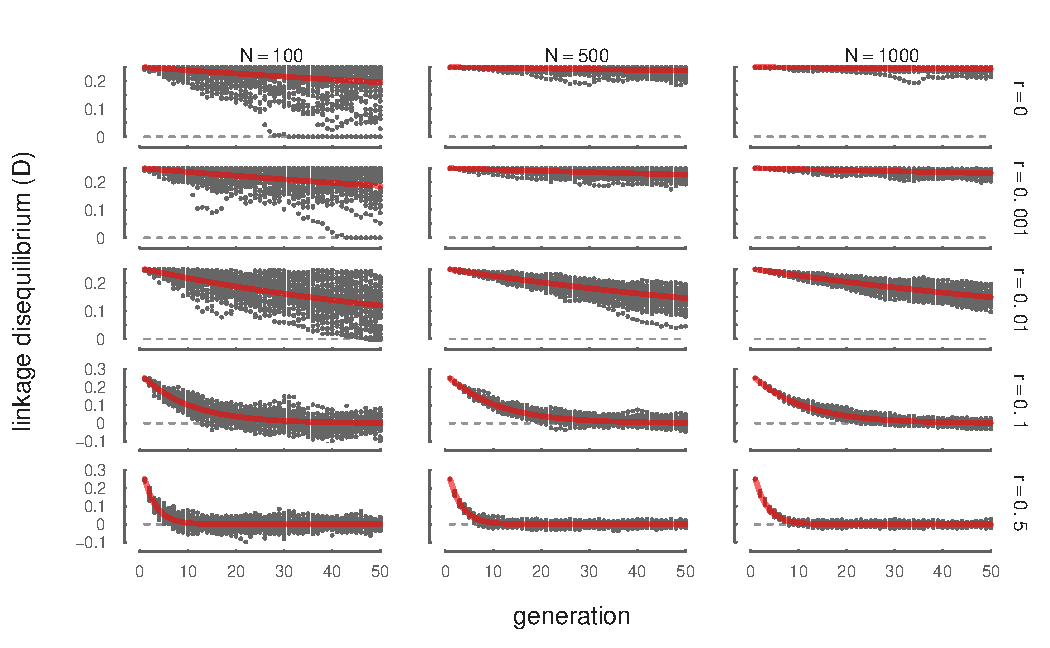
\includegraphics{./images/supp-ld-neutral.pdf}

  \caption{The decay of LD between neutral sites due to recombination, across
    100 replicates and a variety of $V_A$ and $R$ levels. The initial
    population is created to have an artificial level of initial LD, with half
    the gametes carrying all derived alleles, and the other half carrying all
  ancestral alleles. The red line is the theoretical expectation $D_t = D_1 (1-1/(2N))^{t-1} (1-r)^{t-1}$.}

  \label{fig:ld-neut}
\end{figure}


\begin{figure}[!ht] \centering
  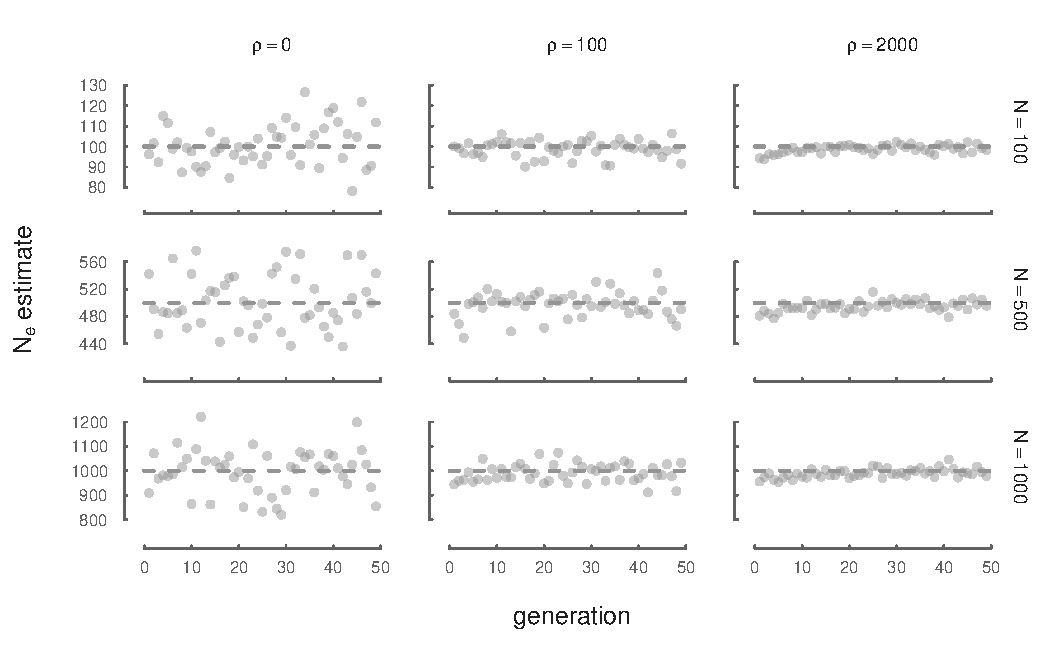
\includegraphics{./images/supp-Ne-est-neutral.pdf} 
  
  \caption{$N_e$ estimated through time from neutral forward simulations is
  consistent with true $N$ across a variety of recombination $\rho$ and $N$
parameters. Here, we estimate $N_e$ with $\widehat{N_e} = \nicefrac{p(1-p)}{2
\var(\Delta p)}$ from neutral allele frequency changes.}

  \label{fig:ne-neut}
\end{figure}

\clearpage
\newpage

\section{Dynamics of Variances}

\begin{figure}[!ht]
  \centering
  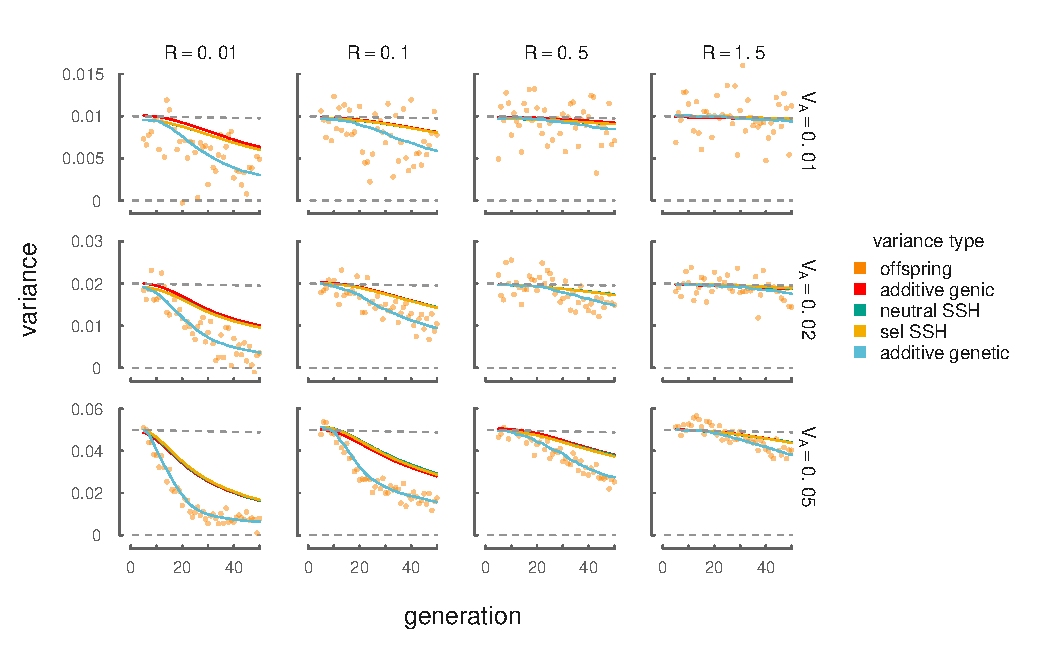
\includegraphics{./images/expfit-vark-types.pdf}
  \caption{The dynamics of different variances in our simulations, across a
    variety of initial target $V_A$ and $R$ levels. Orange points represent the
    empirical heritable variance in offspring (e.g. with the noise of the
    Wright--Fisher reproduction process removed). These closely track the
    additive genetic variance for the trait undergoing directional selection,
    $V_A = \var(z)$. The red line shows the dynamics of additive genic
    variance, $V_a = 2 \sum_l \alpha_l^2 p_l(1-p_l)$, which is closely tracked
  by both the selected (yellow line) and neutral (green line) sum of site
heterozygosity proxies described in Section \ref{sec:dyn-var}.}

  \label{fig:multilocus-expfit-vark}
\end{figure}

\clearpage
\newpage

\section{Supplementary Temporal Autocovariance Figures}

\begin{figure}[!ht]
  \centering
  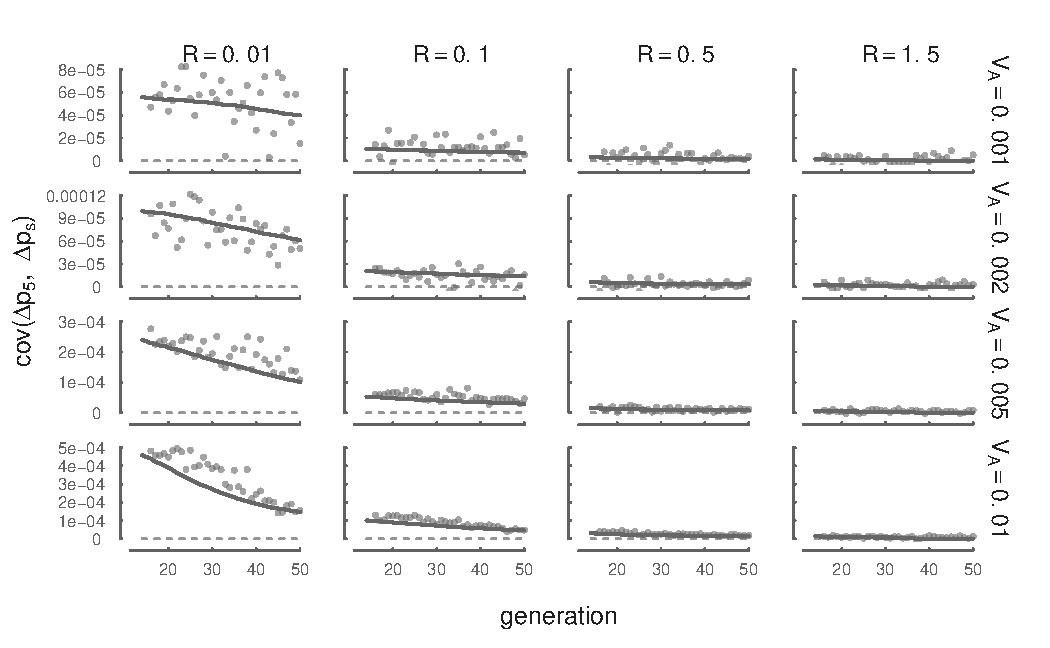
\includegraphics{./images/sim-pred13-covs-varyl.pdf}
  \caption{Each panel shows the temporal autocovariance $\cov(\Delta p_{13},
    \Delta p_s)$ on the y-axis, where $s$ varies along the x-axis. This is
    analogous to Figure \ref{fig:multilocus-expfit-sims} with a different
    reference generation ($t=13$), and compares the averaged simulation results
    (points) with the temporal autocovariance predicted by Equation
    \eqref{eq:multilocus-triangle} using the empirical additive genetic
    variance (curve). The covariances in these panels are weaker compared
    to those in Figure \ref{fig:multilocus-expfit-sims} because by generation
    13, additive genetic variance for fitness and the linkage disequilibria
    between neutral and selected sites has decayed.
}

\label{fig:multilocus-expfit-sims-gen13} 
\end{figure}


\begin{figure}[!ht]
  \centering
  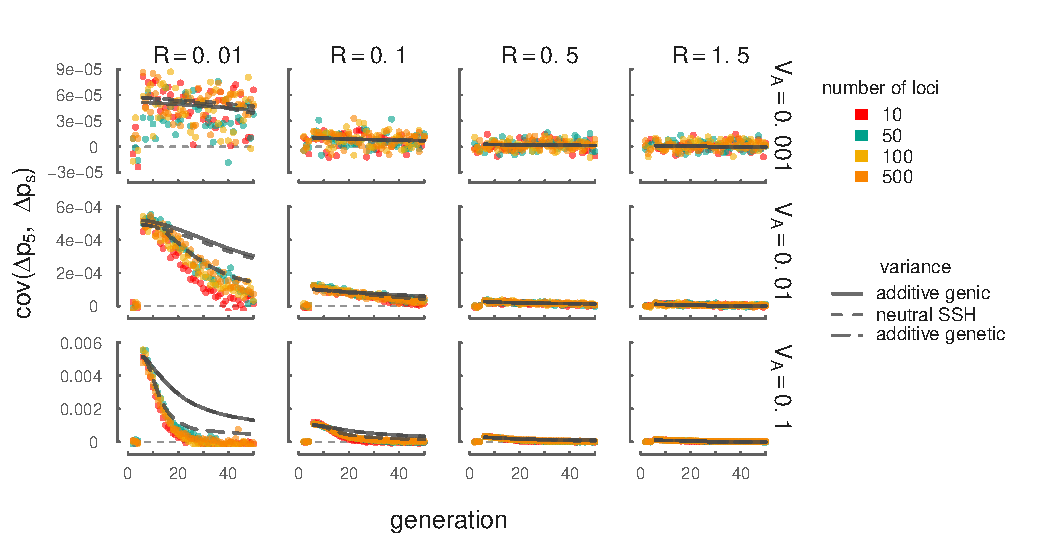
\includegraphics{./images/sim-pred-covs-varyl-va-oom.pdf}

  \caption{A version of Figure \ref{fig:multilocus-expfit-sims} with a subset
    of $V_A$ parameters used in our simulations that vary over orders of
    magnitude. This demonstrates that our theory using the empirical additive
    genic variance (solid gray line), additive genetic variance (long dashed
    gray line), and the neutral SSH proxy (short dashed gray lines) performs as
    described in Section \ref{sec:ml-sim-res} even when $V_A$ varies over
    orders of magnitude in a region. Higher variance in the empirical
    covariances with weak selection ($V_A = 0.001$) are due to chance covariances
    due to drift. The light gray dashed line depicts $\cov(\Delta p_5, \Delta p_s) =
  0$.}
  

  \label{fig:multilocus-expfit-sims-va-oom}
\end{figure}

\begin{figure}[!ht]
  \centering
  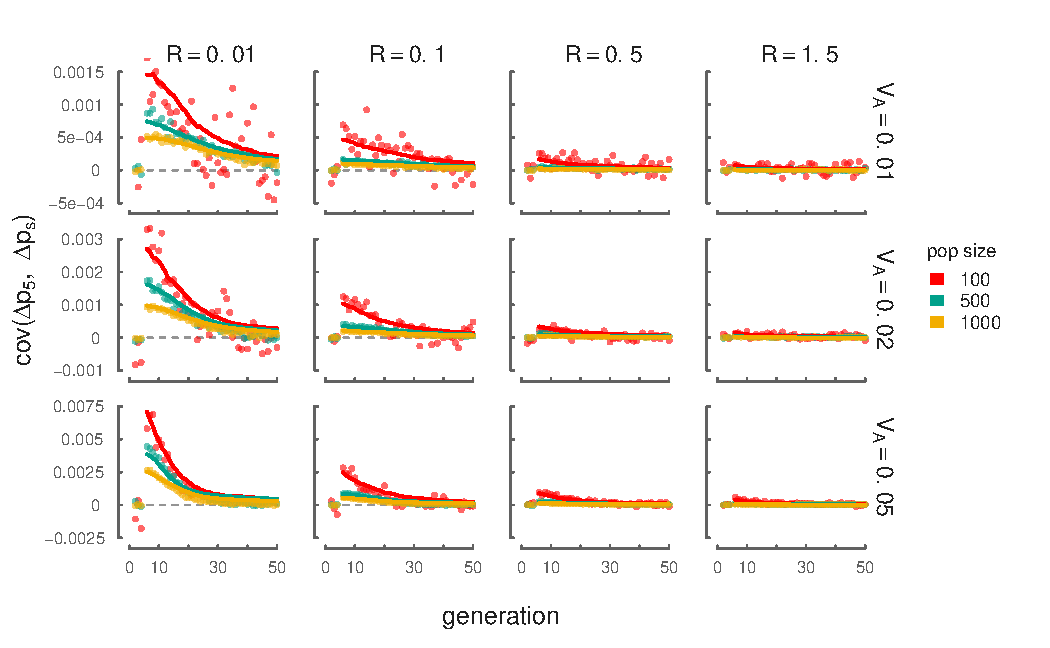
\includegraphics{./images/sim-pred-covs-varyn.pdf}

  \caption{A version of Figure \ref{fig:multilocus-expfit-sims} demonstrating
    temporal autocovariance simulation results and theoretical predictions with
    varying $N$. This demonstrates that our theory using the empirical additive
    genetic variance (lines) fits simulations across a variety of $N$
    parameters.  The light gray dashed line depicts $\cov(\Delta p_5, \Delta p_s) =
  0$. Note that the initial LD varies due to differing equilibrium levels of
LD from our burnin across varying $N$.}

  \label{fig:multilocus-expfit-sims-varyn}
\end{figure}


\end{document}
